% TEMPLATE for Usenix papers, specifically to meet requirements of
%  USENIX '05
% originally a template for producing IEEE-format articles using LaTeX.
%   written by Matthew Ward, CS Department, Worcester Polytechnic Institute.
% adapted by David Beazley for his excellent SWIG paper in Proceedings,
%   Tcl 96
% turned into a smartass generic template by De Clarke, with thanks to
%   both the above pioneers
% use at your own risk.  Complaints to /dev/null.
% make it two column with no page numbering, default is 10 point

% Munged by Fred Douglis <douglis@research.att.com> 10/97 to separate
% the .sty file from the LaTeX source template, so that people can
% more easily include the .sty file into an existing document.  Also
% changed to more closely follow the style guidelines as represented
% by the Word sample file. 

% Note that since 2010, USENIX does not require endnotes. If you want
% foot of page notes, don't include the endnotes package in the 
% usepackage command, below.

% This version uses the latex2e styles, not the very ancient 2.09 stuff.
\documentclass[letterpaper,twocolumn,10pt]{article}
\usepackage{endnotes}
\usepackage{alltt}
\usepackage{url}
\usepackage{amsfonts}
% Type1 fonts please!
\usepackage{amsmath}
\usepackage[T1]{fontenc}
%\usepackage{times,courier,mathptmx}
\usepackage{pifont}
\usepackage{times}
\usepackage{textcomp}
\usepackage{graphicx}
%\usepackage{amsmath,amsthm}
\usepackage{epsfig}
\usepackage{cite}
%\usepackage{color}
\usepackage[table]{xcolor}
\usepackage{xspace}
%\usepackage[tight]{subfigure}
\usepackage{mathspec}
\usepackage[subrefformat=parens,labelformat=parens]{subfig}
\setmainfont[Ligatures=TeX,BoldFont={Minion Pro Bold}, 
 ItalicFont={Minion Pro Italic},
 BoldItalicFont={Minion Pro Bold Italic}]{Minion Pro}
\setmathrm{Minion Pro} 
\setmathfont{Minion Pro}
\setmathfont(Digits,Latin){Minion Pro}
\begin{document}

\newcommand{\notegk}[1]{\textcolor{red}{[G: #1]}}
\newcommand{\noteion}[1]{\textcolor{blue}{[I: #1]}}
%don't want date printed
\date{}

%make title bold and 14 pt font (Latex default is non-bold, 16 pt)
\title{\huge \textit{Title}}

%for single author (just remove % characters)
\author{
{\rm Gautam Kumar}\\
UC Berkeley
\and
{\rm Sylvia Ratnasamy}\\
UC Berkeley
\and
{\rm Ion Stoica}\\
UC Berkeley
} % end author

\maketitle

% Use the following at camera-ready time to suppress page numbers.
% Comment it out when you first submit the paper for review.
%\thispagestyle{empty}


\subsection*{Abstract}
Your Abstract Text Goes Here.  Just a few facts.
Whet our appetites.

\section{Introduction}
Internet services follow strict real-time constraints. 
Services running on large-amount of data leverage massive parallelism to achieve these deadlines. 
This gives rise to a partition-aggregate workflow where a particular request is handled by thousands of machines, 
each one of them operating on a single shard of data and the responses are aggregated in a hierarchical fashion 
before computing the final response for the request. 
This results in two types of deadlines. 
The real-time constraints impose a soft-deadline over the entire workflow and this latency target is subject to optimization. 
The aggregation stages are encumbered by hard deadlines that denote how long should they wait to collect all the sub-responses
before sending the results up in the hierarchy. 


\begin{figure*}[t]
  \centering
  \subfloat
  {
    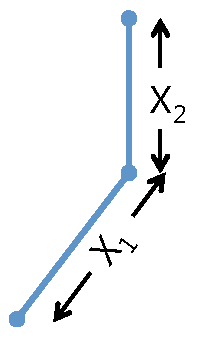
\includegraphics[width=1in]{Figures/2Stage.pdf}
    \label{figure:2StageSimple}
  }
  \hspace{0.5in}
  \subfloat
  {
    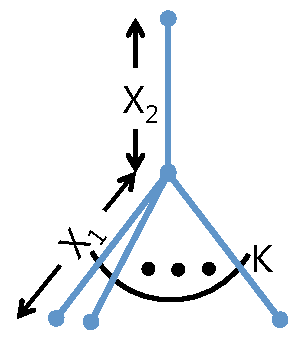
\includegraphics[width=1.5in]{Figures/2StageAggregation.pdf}
    \label{figure:2StageAggregation}
  }
  \hspace{0.5in}
    \subfloat
  {
    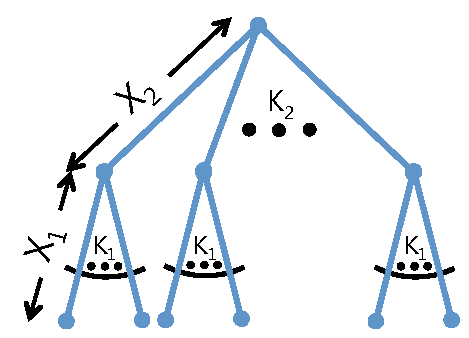
\includegraphics[width=2.5in]{Figures/2StageAggregationFull.pdf}
    \label{figure:2StageAggregationFull}
  }
    \caption{A simple two-stage pipeline. (a) Without aggregation (b) With aggregation at the first stage (c) With aggregation at both the stages.}
  \label{figure:2Stage}
\end{figure*}



\section{Theory}
Consider a simple two-stage pipeline as shown in Figure~\ref{figure:2Stage}. 
Figure~\ref{figure:2StageSimple} denote the two stages in the pipeline without any aggregation. 
Let $X_1$ and $X_2$ be random variables denoting the time taken in the first and the second stages of the pipeline respectively. 
The CDF for $X_1$ is denoted by $\phi_{X_1}(t)$ which is equal to the probability, $\mathbb{P}[X_1 \leq t]$, and the corresponding density function given by $p_1(t)$.
The distribution for the end-to-end response time is given by the $Y = X_1 + X_2$ whose CDF, denoted by $\phi_{Y}(t)$, is given by:
$$
\phi_Y(t) = \int_{y = 0}^t \ \int_{x_1 = 0}^{y} p_1(x_1) \  p_2(y - x_1) \ dx_1 \  dy
$$
For the sake of simplicity, let us assume that $X = X_1 = X_2$. If $X$ is exponentially distributed with parameter $\lambda$, then $\phi_Y(t) = (1 - (1 + \lambda t) e^{-\lambda t})$
with $p_Y(t) = \lambda^2 t e^{-\lambda t}$.

%When the responses from the first stage are aggregated, the time that the first stage takes is distributed as per $X_1' = \textsf{max}(X_1^1, X_1^2, \dots, X_1^k)$. 
%The end-to-end response time variation is then given by, $Z = X_1' + X2$. 
%If $X_1$ is exponentially distributed, as above, then $\phi_{X_1'}(t)$ is given by $(1 - e^{-\lambda t})^k$ with $p_{X_1'} = k\lambda(1 - e^{-\lambda t})^{k- 1}e^{-\lambda t}$.
%The CDF, $\phi_Z(t)$ is given by:
%$$
%\phi_Z(t) = \int_{z = 0}^t \ \int_{x_1' = 0}^{y} p_1(x_1') \  p_2(z - x_1') \ dx_1' \  dz
%$$
%which becomes the integral of an incomplete Beta function.

The exponential distributions reflect the long tail in task durations that occur in typical data center applications. 
The aggregator needs to wait for all the responses to come back before ranking them and sending them up the chain. 
Since this operates under the regime of tight latency targets, if all the responses do not come back in time, the aggregator may decide to leave some of them and rank the partial set of responses thereby degrading the quality\footnote{We use a generic term, information content, to denote the quality of the result. \notegk{To fix.}}. We ask the following question - Given a budget, $D$, for the end-to-end latency, how much should individual stage aggregators wait before sending their partial result up the chain.

Consider the aggregator stage having waited for $t$ units of time and has not received all the responses.
The question then is whether it should wait for an additional $\Delta t$ time or not. 
There is a non-zero probability that it receives additional responses in this time, but this comes at the expense of increased probability of missing the latency target, or worse, getting missed by the aggregator at the above stage, rendering that branch of computation wasted.
We formalize the tradeoff between the quality of result and the deadline target as follow. 
To the best of our knowledge, we are the first to undertake a analysis of such workflow and the formalism that follows. \\
Given that the aggregator has waited for $t$ units of time, the probability \textsf{Pr}[A new response is received in $\Delta t$ | Elapsed time $= t$] = $1 - $\textsf{Pr}[No new response arrives in $\Delta t$ | Elapsed time $= t$] = $1 - \left[1 - (\phi_{X_1}(t + \Delta t) - \phi_{X_1}(t)) \right] ^k$. 
Denote $N(t)$ to be the random variable denoting the number of responses received uptil time $t$. 
One can see that $N(t)$ is binomial with success probability $ = \phi_{X_1}(t)$. 
The expected number of responses received by time $t$, given by $\mathbb{E}[N(t) = k\phi_{X_1}(t)$.
For exponentially distributed $X_1$, this is given by $k(1 - e^{-\lambda t})$. 
These set of responses contribute to the final result if the aggregator meets the deadline $D$ of the above stage which happens with probability $\phi_{X_2}(D - t)$. 
Thus while $\mathbb{E}[N(t)]$ is an increasing function in $t$, the probability that those set of responses make it in time to be aggregated by the top level decreases with time.
If lost, the entire branch of computation is lost. It is important for internet services to deliver all the responses, and the quality of query is of utmost importance. 
Thus one can write the Utility function, $U(t)$, as $\mathbb{E}[N(t)]\phi_{X_2}(D - t) = k\phi_{X_1}(t)\phi_{X_2}(D - t)$. 
If $X_1$ and $X_2$ are exponentially distributed, then $U(t)$ = $k(1 - e^{-\lambda_1 t})(1 - e^{-\lambda_2(D - t)})$.
The function being concave exhibits a distinct maxima when $U'(t) = k\left(\phi_{X_1}'(t)\phi_{X_2}(D - t) - \phi_{X_1}(t)\phi_{X_2}'(D - t)\right) = 0$
Two important points surface, one is that this timeout selection is independent of the fanout degree, $k$. 
Even if the expected utility small, one can make the most out of it.
The curve becomes flatter as one increases the latency budget.

\begin{figure}[t]
\centering
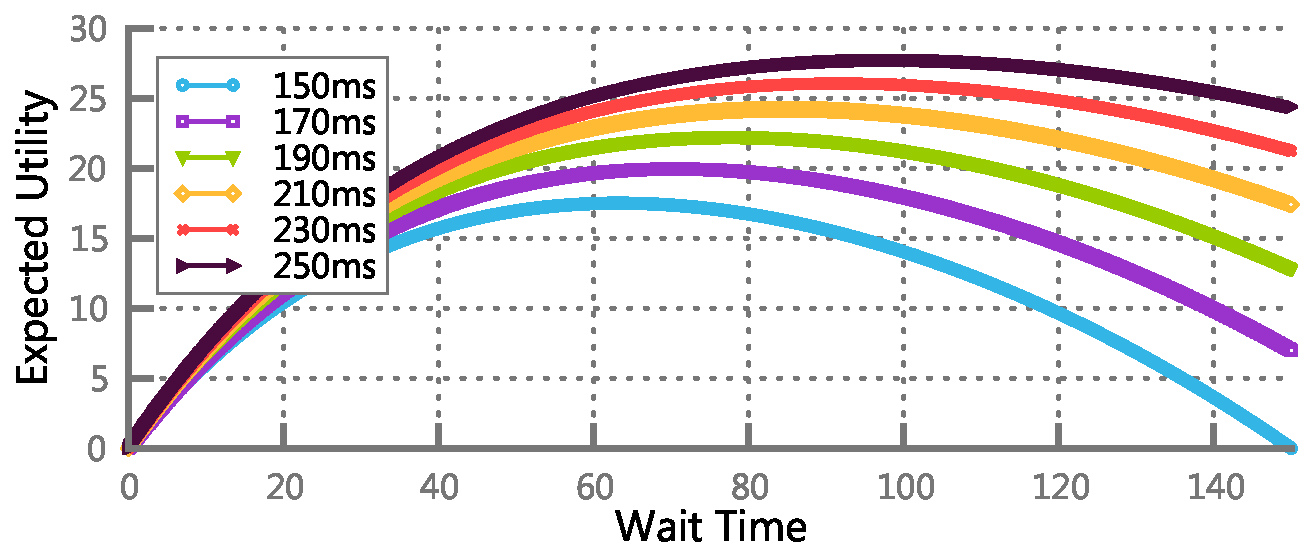
\includegraphics[width=3.2in]{Matplotlib/UtilityAnalytical.pdf}
\label{figure:UtilityAnalytical}
\caption{\small For exponentially distributed $X_1$ and $X_2$, with mean 45ms and 100ms respectively, the utility function values as a function of wait time $t$ for different deadline, $D$, values.}
\end{figure}


Let $X_1$ have a mean of 45ms and $X_2$ have a mean of 100ms\notegk{Numbers from D3}. 
Figure~\ref{figure:UtilityAnalytical} shows the the variation of the expected utility with respect to the wait time at the aggregator node for different deadline values. 


{\footnotesize \bibliographystyle{acm}
\bibliography{../common/bibliography}}


\theendnotes

\end{document}






